\subsection{Estado, recurrencia y complejidad}
Se define $F(i,j,\ell)$ como el mayor puntaje de un camino que alcanza
$(i,j)$ con exactamente $\ell\in\{1,\ldots,V\}$ vidas. Los estados
inalcanzables valen $-\infty$ y $F(1,1,V)=g_{1,1}$. Para las demás celdas:
\[
F(i,j,\ell)=
\begin{cases}
\max\{F(i-1,j,\ell),F(i,j-1,\ell)\}+g_{i,j}, & t_{i,j}=1,\\
\max\{F(i-1,j,\ell+1),F(i,j-1,\ell+1)\}-P, & t_{i,j}=-1,\ \ell<V,\\
-\infty, & \text{en otro caso}.
\end{cases}
\]
Los índices fuera de la grilla representan estados inalcanzables. La
respuesta es $\max_{1\leq\ell\leq V}F(N,M,\ell)$. No se descartan puntajes
negativos ni se permite llegar a cero vidas. Un camino válido termina
necesariamente desde arriba o desde la izquierda. Si un prefijo no fuera
óptimo para su celda y sus vidas, reemplazarlo por el mejor prefijo
conservaría la validez y mejoraría el puntaje total. Esto justifica la
recurrencia. La implementación propaga los estados en orden de filas,
guarda el movimiento predecesor y reconstruye desde el destino; al
retroceder sobre una mina se recupera una vida. Esta formulación sigue los
principios de programación dinámica descritos por Roughgarden~\cite{roughgarden2019algorithms}.

Con $L=N+M-2$ y $C=\binom{L}{N-1}$, fuerza bruta examina todos los
prefijos válidos, con cota temporal $O(LC)$ y memoria auxiliar $O(L)$.
La copia del mejor camino cuesta $O(L)$ por cada nuevo óptimo. En grillas cuadradas libres,
$C=\binom{2N-2}{N-1}$ crece exponencialmente con $N$.
Las murallas y la pérdida de vidas permiten descartar únicamente ramas
inválidas. DP recorre $NMV$ estados con hasta dos transiciones por estado:
tiempo y espacio auxiliar $\Theta(NMV)$, más reconstrucción $O(L)$.
Greedy hace hasta $L$ decisiones de costo constante y almacena su camino:
tiempo y espacio auxiliar $O(N+M)$. DP y greedy validan las dimensiones en
$O(N)$; fuerza bruta recibe grillas válidas y no comprueba esas dimensiones.
La lectura y las matrices de
entrada añaden $\Theta(NM)$ al tiempo total y al espacio de los tres
programas, aunque la lectura no entra al cronómetro.

\subsection{Tiempo y memoria}
DP encontró solución en las 288 instancias y coincidió en existencia y
puntaje con fuerza bruta en los 120 casos con $N+M\leq32$. Se validaron
los 658 caminos encontrados (120 de fuerza bruta, 288 de DP y 250 de
greedy), recalculando longitud, movimientos, puntaje y vidas. Las rutas
óptimas pueden diferir al empatar, sin alterar el resultado exigido.
La Tabla~\ref{tab:costos} resume las medias de 24 instancias por tamaño;
los guiones indican que fuerza bruta no se ejecutó por la restricción del
enunciado, no que su tiempo fuese cero.

\begin{table}[H]
\centering\footnotesize
\begin{tabular}{lrrrrr}
\hline
$N\times M$ & BF (ms) & DP (ms) & Greedy (ms) & DP (MiB) & Greedy (MiB) \\
\hline
$4\times4$ & 0.0011 & 0.0050 & 0.0003 & 5.19 & 5.19 \\
$8\times16$ & 3.7378 & 0.0282 & 0.0005 & 5.23 & 5.20 \\
$16\times16$ & 3152.6367 & 0.0463 & 0.0007 & 5.24 & 5.20 \\
$256\times256$ & -- & 12.3114 & 0.0094 & 13.27 & 6.06 \\
$1024\times1024$ & -- & 207.7318 & 0.0631 & 130.45 & 17.69 \\
$1024\times2048$ & -- & 431.9131 & 0.0877 & 255.22 & 29.80 \\
\hline
\end{tabular}

\caption{Medias de tiempos del solver y máximo residente total. BF: fuerza bruta.}
\label{tab:costos}
\end{table}

La Figura~\ref{fig:costos} muestra el aumento combinatorio de fuerza
bruta: de $8\times16$ a $16\times16$ su media pasa de 3.74 ms a 3152.64 ms,
aunque el área solo se duplica. En $4\times4$, DP resulta más lento por
el costo de crear sus tablas; desde $8\times8$ supera a fuerza bruta en
la media del conjunto. En las grillas grandes DP aumenta aproximadamente
con el área: de $1024\times1024$ a $1024\times2048$ pasa de 207.73 a
431.91 ms (factor 2.08 para el doble de celdas), consistente con
$\Theta(NMV)$ al fijar $V=3$. Los dominios cambian los puntajes pero no
el número de estados. Las diferencias por tipo se muestran en
\texttt{execution\_time.png}: las murallas pueden acortar fuertemente el
DFS, mientras DP sigue inicializando las tablas completas.

\begin{figure}[H]
\centering
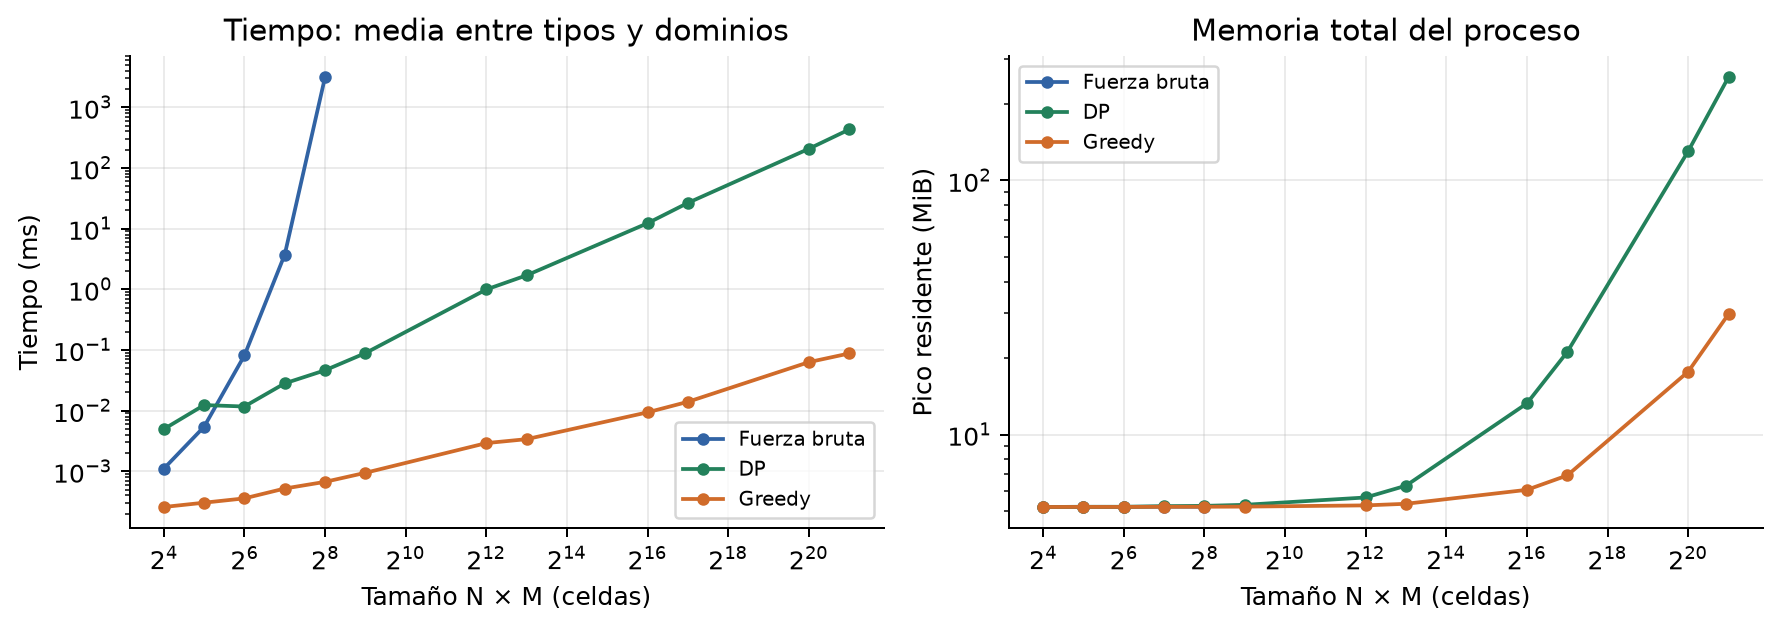
\includegraphics[width=\textwidth]{../code/grid_pathfinding/data/plots/cost_comparison.png}
\caption{Costos medios según el área, con ambos ejes logarítmicos.
El salto de fuerza bruta se observa aun en sus tamaños restringidos.}
\label{fig:costos}
\end{figure}

Greedy tarda 0.0877 ms en promedio en $1024\times2048$, pero su menor
tiempo no implica una solución óptima. Además, una falla puede terminar
el recorrido antes de completar los $L$ pasos: sus tiempos mezclan éxitos
y fallas. Con $M=N$ o $2N$, un recorrido completo es del orden de
$\sqrt{NM}$ al graficar contra el área, mientras DP es lineal en ella.
Los tiempos de las instancias pequeñas son de microsegundos y tienen
ruido relativo considerable; no se interpreta cada oscilación como un
cambio de complejidad.

En memoria, la base del proceso ronda 5.2 MiB y oculta las diferencias en
grillas pequeñas. En $1024\times2048$, DP alcanza 255.22 MiB y greedy
29.80 MiB. La memoria de greedy también crece porque el proceso conserva
ambas matrices completas; esto no contradice su espacio auxiliar
$O(N+M)$. DP agrega dos tablas tridimensionales y las reservas de los
\texttt{vector} anidados. Su máximo casi se duplica en los dos tamaños
mayores, como predice la dependencia en $NMV$. La memoria de fuerza bruta
permanece cercana a la base en los tamaños permitidos; no se midió su
crecimiento para instancias mayores. Estos máximos incluyen entrada y
runtime y no permiten aislar exactamente los bytes auxiliares de cada
algoritmo. Los detalles por tipo están en \texttt{memory\_usage.png}.

\subsection{Calidad de greedy}
Se calcula $\Delta=s(\mathrm{DP})-s(\mathrm{Greedy})$ solo cuando ambos
encuentran camino. No se asigna brecha cero a las fallas ni se usa una
razón de puntajes, que sería engañosa con valores negativos o nulos.
Greedy falla en 38 de 288 casos ($13.19\%$); de sus 250 éxitos, 38
alcanzan el óptimo ($15.2\%$). La Tabla~\ref{tab:calidad} reúne las 36
instancias de cada combinación de tipo y dominio; sus brechas medias
mezclan tamaños y deben leerse junto con la Figura~\ref{fig:calidad}.

\begin{table}[H]
\centering\small
\begin{tabular}{llrrr}
\hline
Tipo & Dominio & Fallas / casos & Fallas (\%) & $\overline{\Delta}$ (éxitos) \\
\hline
Libre & D10 & 0/36 & 0.0 & 1204.1 \\
Libre & D1000 & 0/36 & 0.0 & 121868.0 \\
Murallas & D10 & 8/36 & 22.2 & 1145.1 \\
Murallas & D1000 & 12/36 & 33.3 & 132598.6 \\
Minas & D10 & 0/36 & 0.0 & 1199.3 \\
Minas & D1000 & 1/36 & 2.8 & 122789.1 \\
Mixta & D10 & 12/36 & 33.3 & 965.9 \\
Mixta & D1000 & 5/36 & 13.9 & 110891.2 \\
\hline
\end{tabular}

\caption{Fallas sobre todas las instancias; brecha media condicionada al éxito.}
\label{tab:calidad}
\end{table}



En grillas libres greedy siempre llega a la meta, pero pierde calidad
por elegir ganancias inmediatas: su brecha crece con el tamaño en ambos
dominios. Las minas permiten el paso a cambio de vida y puntaje; greedy
solo falló una vez en este tipo (D1000), y ninguna en D10. Las murallas
sí impiden entrar, de modo que una elección local puede conducir a un
callejón sin salida aunque exista el camino reservado. Se observan 20
fallas con murallas y 17 en mixtas. La mezcla no es siempre peor en esta
muestra: en D10 falla 12/36 veces frente a 8/36 con murallas, mientras en
D1000 falla 5/36 frente a 12/36. Son terrenos aleatorios distintos, no
pares idénticos para atribuir causalmente esa diferencia al dominio.

Solo hay tres muestras por tamaño, tipo y dominio: las tasas avanzan en
pasos de $33.3\%$ y no estiman con precisión una población.
El aumento del tamaño no produce una tasa de falla monótona. Por ejemplo,
en $8\times16$ las tres mixtas D10 fallan, mientras en $256\times256$
ninguna de esas tres falla. La cantidad de obstáculos es
$K=\lfloor\sqrt{NM}\rfloor$ por clase; su densidad disminuye con el área,
y la reserva de un camino seguro condiciona las posiciones posibles.
Por ello estos resultados no describen terrenos de densidad constante.
En D1000 las brechas tienen una escala aproximadamente cien veces mayor
que en D10, coherente con el rango de valores y la penalización. No
representan una pérdida relativa cien veces mayor. Las gráficas usan
ejes verticales separados y no prueban proporcionalidad exacta, porque
los mapas y valores se generan de forma independiente.

\begin{figure}[H]
\centering
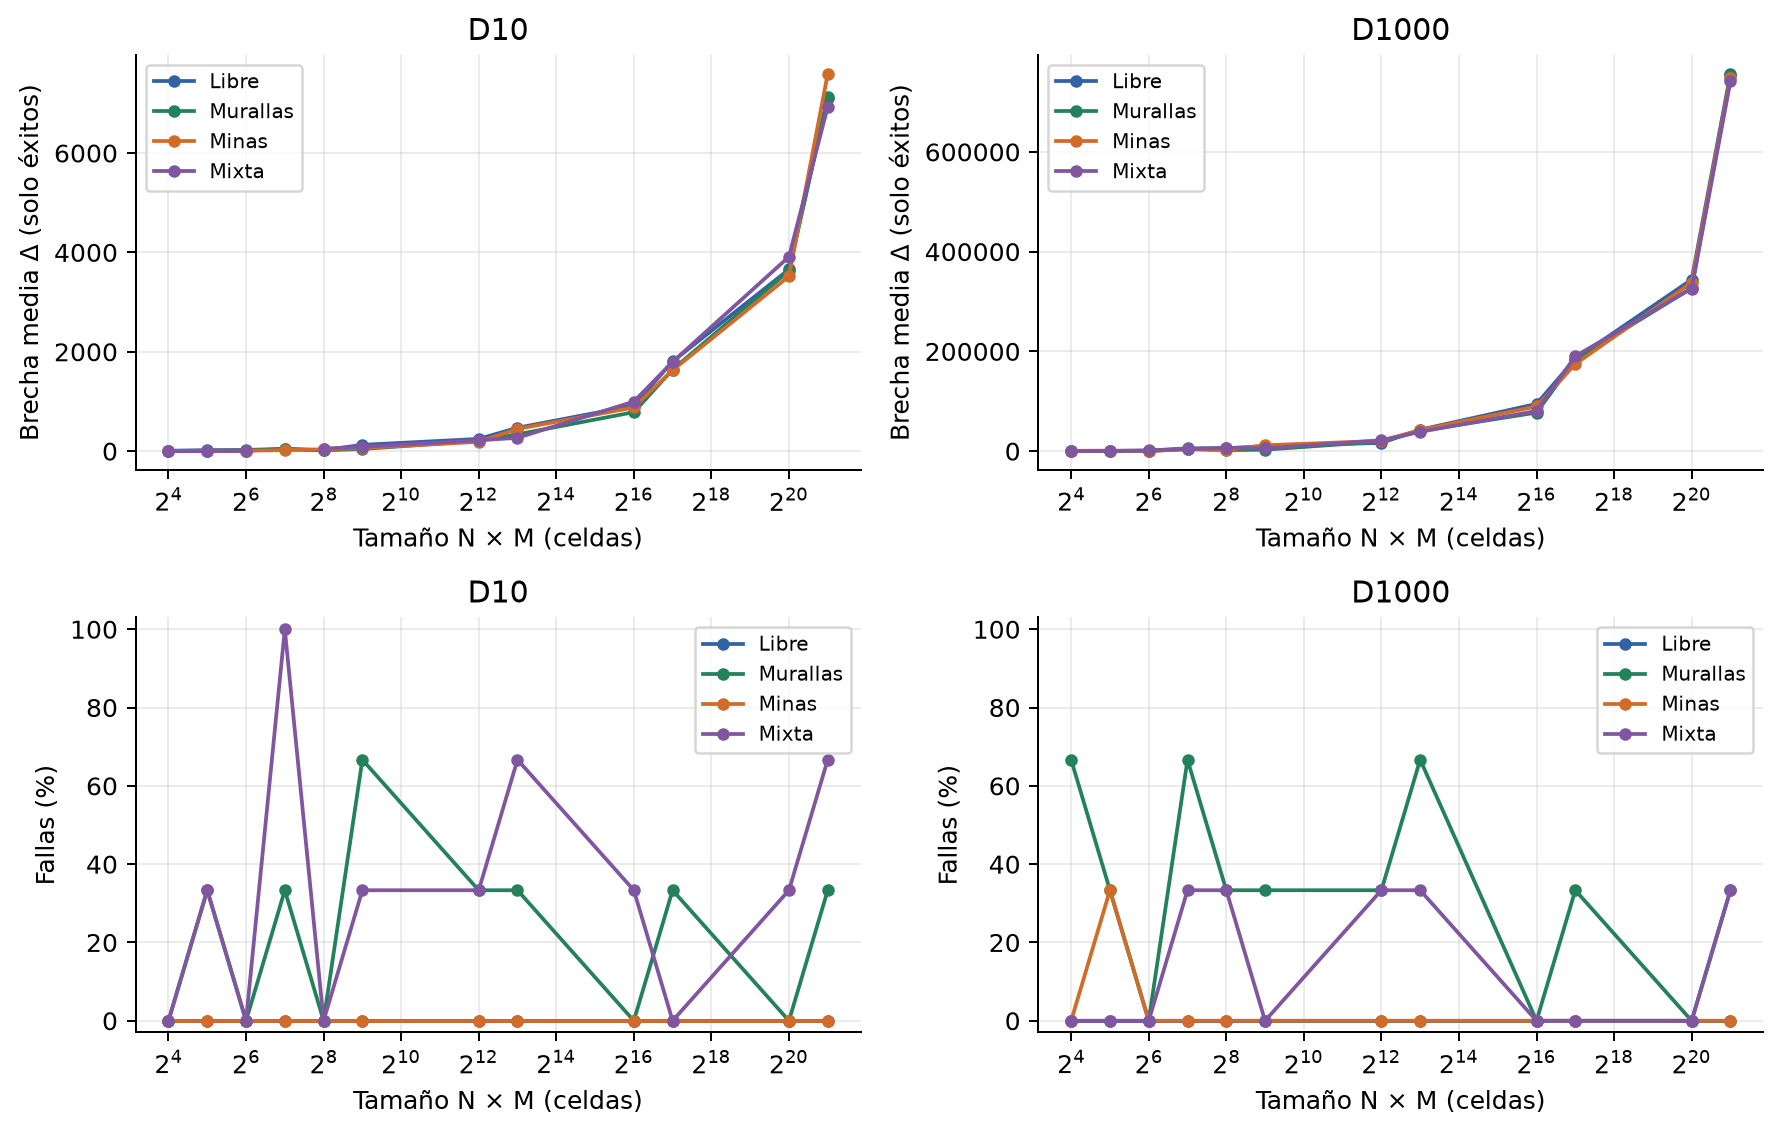
\includegraphics[width=\textwidth]{../code/grid_pathfinding/data/plots/greedy_quality.png}
\caption{Brecha y fallas por área, tipo y dominio. Cada punto resume tres
muestras. Una brecha ausente indica que no hubo éxitos en ese grupo;
las líneas entre tamaños solo facilitan la lectura.}
\label{fig:calidad}
\end{figure}

\subsection{Reproducción y alcance}
El programa principal compara BF/DP y registra medidas en
\path{main_results.csv}. El auxiliar \path{run_measurements.py} mide cada
algoritmo por separado, comprueba sus resultados y genera \path{results.csv}.
\path{plot_generator.py} y \path{generate_report_tables.py} leen ese CSV para
regenerar figuras y tablas. Los pasos están en \path{code/README.md}. Se
conservan los algoritmos BF y greedy y las salidas del programa; el principal
agrega la comparación y las medidas. Como solo varían $N,M$ y $V=3$, el
experimento no permite medir por separado la dependencia en $V$.
Los resultados corresponden a esta semilla, este equipo y este esquema
de repetición; especialmente en los grupos con pocos éxitos, una brecha
media pequeña no permite concluir que el algoritmo sea más confiable.
